\documentclass[11pt]{article}
\usepackage{amsmath}
\usepackage{amssymb}
\usepackage{xparse}
\usepackage{listings}
\usepackage{color}
\usepackage{graphicx}
\usepackage[a4paper, total={6in, 8in}, voffset=0in]{geometry}



\definecolor{codeblue}{rgb}{0.3,0.4,0.9}
\definecolor{codegreen}{rgb}{0,0.5,0}
\definecolor{codegray}{rgb}{0.5,0.5,0.5}
\definecolor{codepurple}{rgb}{0.58,0,0.82}
\definecolor{backcolour}{rgb}{0.95,0.95,0.92}
 
\lstdefinestyle{mystyle}{
    backgroundcolor=\color{backcolour},   
    commentstyle=\color{codegray},
    keywordstyle=\color{codeblue},
    stringstyle=\color{codegreen},
    basicstyle=\footnotesize,
    breakatwhitespace=false,         
    breaklines=true,                 
    captionpos=b,                    
    keepspaces=true,                                    
    numbersep=5pt,                  
    showspaces=false,                
    showstringspaces=false,
    showtabs=false,                 
    tabsize=2
}
 
\lstset{style=mystyle}

\begin{document}
\begingroup  
  \centering
  \LARGE CMSC498F Final\\[.5em]
  \large Simon Milburn\\[.5em]
  \large \today\\[.5em]
  \noindent\rule[0.5ex]{\linewidth}{1pt}
   \large \\ [2em]
\endgroup

	\begin{enumerate}
	
	\item[\textbf{1}] 
		Given two observations $\hat{q}_1$ and $\hat{q}_2$ with variances 		
		$\sigma_1^2$ and $\sigma_2^2$ of a normal distributed process
		with actual value $\hat{q}$. The optimal estimate can be calculated by minimizing the expression
		\[
   			 S = \frac{1}{\sigma_1^2}(\hat{q}-\hat{q}_1)^2 +  \frac{1}{\sigma_2^2}(\hat{q}-\hat{q}_2)^2
		\]
		Calculate $\hat{q}$ so that $S$ is minimized.
		
	\item[\textbf{2}] 
		 An ultrasound sensor measures distance x =$\frac{c\Delta t}{2}$. Here, $c$ is the speed of sound and $\Delta t$ is the
		difference in time between emitting and receiving a signal.
		\begin{enumerate} 
			\item Let the variance of your time measurement $\Delta t$ be $\sigma_t^2$. What can you say about the 	
			variance of $x$, when $c$ is assumed to be constant? Hint: how does a change in $\Delta t$ affect $x$?
			
			\item Now assume that also $c$ is changing depending on location, weather, etc. and can be estimated
			with variance $\sigma_c^2$. What is the variance of $x$ now?
		\end{enumerate}
		
	\item[\textbf{3}] 
		 SIFT feature description and detection
		\begin{enumerate} 
			\item Describe the four computational steps of SIFT feature description and detection.
			\item Describe SURF features, and discuss how and why the computations of these features are
			more efficient than SIFT
			\item Describe one other feature detector from the literature.
		\end{enumerate}
		
	\item[\textbf{4}] 
		Assume the following scene shown in Fig.1 with a background plane of 5m distance and two
		objects (a rounded rectangle and a triangle) at 1m distance as drawn below.
		
		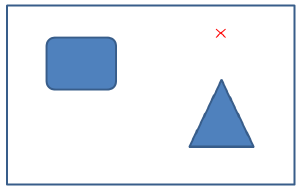
\includegraphics[scale = .85]{scene.png}
		\begin{enumerate} 
			\item The camera is moving towards the scene with the direction of translation denoted by the red
			cross (the so-called Focus of Expansion). Draw the flow field qualitatively.		
			
			\item What is the aperture problem in computing optical flow? How is it related to the linear
			constraint on optical flow (?brightness constraint?) determined by the differential technique for
			computing flow?
			
			\item Describe the Lucas Kanade optical flow algorithm.
		\end{enumerate}
		
	\item[\textbf{5}] 
		Assume that the ceiling is equipped with infra-red markers that the robot can identify with
		some certainty. Your task is to develop a probabilistic localization scheme, and you would like
		to calculate the probability p($marker$|$reading$) to be close to a certain marker given a certain
		sensing reading and information about how the robot has moved. 	
		
		\begin{enumerate} 
			\item Derive an expression
				for p($marker$|$reading$) assuming that you have an estimate of the probability to correctly identify
				a marker p($reading$|$marker$) and the probability p($marker$) of being underneath a specific
				marker.
				
			\item Now assume that the likelihood that you are reading a marker correctly is 90\%, that you
			get a wrong reading is 10\% and that you do not see a marker when passing right underneath it is  			50\%. Consider a narrow corridor that is equipped with 4 markers. You know
			with certainty that you started from the entry closests to marker 1 and move right in a straight
			line. The first reading you get is "Marker 3". Calculate the probability to be indeed underneath
			marker 3.
			
			\item Could the robot also possibly be underneath marker 4?
		\end{enumerate}
	\end{enumerate}	
\end{document}
